\documentclass{beamer}
\usepackage[utf8]{inputenc}
\usepackage[T1]{fontenc}

\usetheme{Cuerna}
\usecolortheme{default}

\logo{
\includegraphics[scale=0.35]{images/freistrom.png}}
\title{Notejam Pilot for Nordcloud}
\author{David Spautz\\
\texttt{david.spautz@freistrom.io}}

\date{February 13. 2021}
\institute{Freistrom, Germany}

\begin{document}

  \begin{frame}
    \titlepage
  \end{frame}

  \section{Introduction}
  \begin{frame}
    \frametitle{The Project}
    \framesubtitle{A Quick Overview}
    \begin{itemize}
    \item First Pilot in Public Cloud
    \item Core Concepts and Architecture
    \item In GCP (Google Cloud Provider)
    \item Notejam - A Simple Webapp to handle notes online
  \end{itemize}
  \end{frame}

  \begin{frame}
  	\frametitle{The Project}
  	\framesubtitle{What is and what should be}
  	\center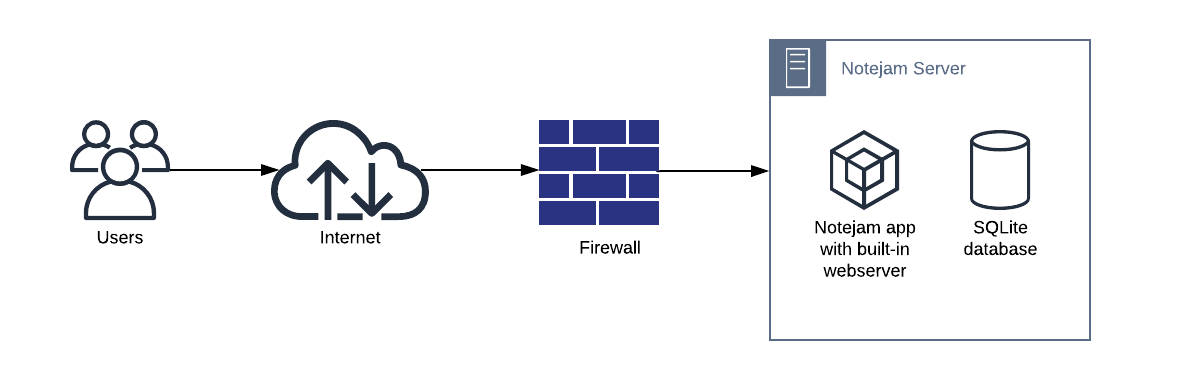
\includegraphics[width=10cm,height=3cm]{images/current_architecture.png}
  	\begin{itemize}
  		\item Separate the Data Tier
  		\item Variable amount of Traffic should be served with peek times
  		\item Notes should be preserve up to 3 years
  		\item Service needs to be failure tolerant
  		\item Multiple Deployments a day by up to 100 developer
  		\item Separate environments (production, testing, development)
  		\item Relevant metrics and logs for the asssurance and security 
  	\end{itemize}
  \end{frame}

\end{document}